\documentclass[a4paper,11pt]{article}
\usepackage[margin=22mm,headheight=15pt,headsep=8mm,footskip=11mm]{geometry}
\usepackage{amsmath,amssymb,booktabs,enumitem,fancyhdr,xcolor,tikz}
\usepackage[unicode,hidelinks]{hyperref}
\hypersetup{pdftitle={Stochastic Signal Analysis - Homework 1 Solutions}}
\pagestyle{fancy}\fancyhf{}
\fancyhead[L]{\small Stochastic Signal Analysis}\fancyhead[R]{\small Homework \#1: Solutions}
\fancyfoot[L]{\scriptsize Companion to the English exercise sheet}\fancyfoot[R]{\small\thepage\ / 11}
\setlength{\parindent}{0pt}\setlength{\parskip}{0.5em}\linespread{1.12}
\newcommand{\E}{\mathbb E}\newcommand{\Var}{\operatorname{Var}}\newcommand{\Cov}{\operatorname{Cov}}
\newcommand{\jj}{\mathrm j}\newcommand{\ee}{\mathrm e}
\newcommand{\problem}[3]{{\LARGE\bfseries Exercise #1}\hfill #2\par{\small\color{gray}Textbook p. #3}\par\vspace{3mm}}
\newcommand{\step}[1]{\par\textbf{#1}\par}
\begin{document}
\problem{1.6}{Required}{34}
Let $B_i$ be the event that batch $i$ is selected, and let $D$ denote a defective component. The batch is selected first, so
\[
P(B_i)=\frac14,\qquad i=1,2,3,4.
\]
The different batch sizes do not change these selection probabilities. Using the stated defect rates,
\[
P(D\mid B_1)=0.05,\quad P(D\mid B_2)=0.40,\quad
P(D\mid B_3)=P(D\mid B_4)=0.10.
\]
\step{(1) Probability of a defective component}
By the law of total probability,
\begin{align*}
P(D)&=\sum_{i=1}^{4}P(D\mid B_i)P(B_i)\\
&=\frac14(0.05+0.40+0.10+0.10)
=\boxed{\frac{13}{80}=0.1625}.
\end{align*}
\step{(2) Probability that a defective component came from batch 2}
By Bayes' theorem,
\[
P(B_2\mid D)=\frac{P(D\mid B_2)P(B_2)}{P(D)}
=\frac{0.40\times\tfrac14}{0.1625}
=\boxed{\frac8{13}\approx0.6154}.
\]
The numerical answers use $10\%$ for the two approximately specified defect rates.
\newpage
\problem{1.14}{Required}{34}
\step{(1) Joint distribution function and density}
The joint CDF is $F_{XY}(x,y)=P(X\le x,Y\le y)$. Summing the given masses gives
\begin{center}\renewcommand{\arraystretch}{1.25}
\begin{tabular}{c|cccc}\toprule
& $y<-1$ & $-1\le y<0$ & $0\le y<1$ & $y\ge1$\\\midrule
$x<0$ &0&0&0&0\\
$0\le x<1$ &0&0.07&0.25&0.40\\
$x\ge1$ &0&0.15&0.65&1\\\bottomrule
\end{tabular}\end{center}
Since the variables are discrete, there is no ordinary joint density. In the generalized (Dirac delta) sense requested by the textbook,
\begin{align*}
f_{XY}(x,y)={}&\delta(x)\bigl[0.07\delta(y+1)+0.18\delta(y)+0.15\delta(y-1)\bigr]\\
&+\delta(x-1)\bigl[0.08\delta(y+1)+0.32\delta(y)+0.20\delta(y-1)\bigr].
\end{align*}
\step{(2) Marginal probability mass functions}
Summing rows and columns,
\[
\boxed{P(X=0)=0.40,\qquad P(X=1)=0.60,}
\]
\[
\boxed{P(Y=-1)=0.15,\quad P(Y=0)=0.50,\quad P(Y=1)=0.35.}
\]
All other marginal masses are zero.
\step{(3) Distribution of $Z=XY$}
$Z=-1$ only at $(1,-1)$; $Z=1$ only at $(1,1)$. All remaining outcomes give $Z=0$. Hence
\[
\boxed{P(Z=-1)=0.08,\quad P(Z=0)=0.72,\quad P(Z=1)=0.20.}
\]
\step{(4) Correlation coefficient}
\[
\E X=0.6,\qquad \E Y=-0.15+0.35=0.2,\qquad
\E(XY)=-0.08+0.20=0.12.
\]
Thus $\Cov(X,Y)=0.12-(0.6)(0.2)=0$. Also,
\[
\Var(X)=0.6-0.6^2=0.24,\qquad
\Var(Y)=0.15+0.35-0.2^2=0.46.
\]
\[
\boxed{\rho_{XY}=\frac{0}{\sqrt{0.24\times0.46}}=0.}
\]
They are uncorrelated but not independent: $P(X=0,Y=-1)=0.07\ne0.40\times0.15$.
\newpage
\problem{1.16}{Required}{35}
Because $X$ and $Y$ are independent standard normal variables,
\[
f_{XY}(x,y)=\frac1{2\pi}\exp\!\left[-\frac{x^2+y^2}{2}\right],
\qquad x,y\in\mathbb R.
\]
\step{(1) Joint density of $U=X+Y$ and $V=X-Y$}
The inverse transformation is
\[
x=\frac{u+v}{2},\qquad y=\frac{u-v}{2}.
\]
Its absolute Jacobian determinant is
\[
\left|\frac{\partial(x,y)}{\partial(u,v)}\right|
=\left|\det\begin{pmatrix}\tfrac12&\tfrac12\\\tfrac12&-\tfrac12\end{pmatrix}\right|
=\frac12.
\]
Since $x^2+y^2=(u^2+v^2)/2$, the change-of-variables formula gives
\[
\boxed{f_{UV}(u,v)=\frac1{4\pi}\exp\!\left[-\frac{u^2+v^2}{4}\right],
\qquad u,v\in\mathbb R.}
\]
\step{(2) Find the marginal densities and test independence}
Integrate the joint density over the other variable:
\begin{align*}
f_U(u)&=\int_{-\infty}^{\infty}f_{UV}(u,v)\,dv
=\frac{\ee^{-u^2/4}}{4\pi}\int_{-\infty}^{\infty}\ee^{-v^2/4}\,dv
=\frac{1}{2\sqrt\pi}\ee^{-u^2/4},\\
f_V(v)&=\int_{-\infty}^{\infty}f_{UV}(u,v)\,du
=\frac{\ee^{-v^2/4}}{4\pi}\int_{-\infty}^{\infty}\ee^{-u^2/4}\,du
=\frac{1}{2\sqrt\pi}\ee^{-v^2/4}.
\end{align*}
Here, substituting $t=v/2$ gives
$\int_{-\infty}^{\infty}\ee^{-v^2/4}\,dv
=2\int_{-\infty}^{\infty}\ee^{-t^2}\,dt=2\sqrt\pi$.
Now compare the product with the joint density:
\[
f_U(u)f_V(v)=\frac{1}{4\pi}\ee^{-(u^2+v^2)/4}=f_{UV}(u,v)
\quad\text{for all }u,v\in\mathbb R.
\]
Thus $U$ and $V$ are independent. Comparing the marginal densities with
$\frac1{\sqrt{2\pi\sigma^2}}\exp[-(z-\mu)^2/(2\sigma^2)]$ also gives
\[
\boxed{U\sim N(0,2),\qquad V\sim N(0,2),\qquad U\text{ and }V\text{ are independent}.}
\]
\newpage
\problem{1.21}{Required}{35}
The given quantities are
\[
\E X=1,\quad\E Y=3,\quad\Var(X)=4,\quad\Var(Y)=16,\quad\rho_{XY}=0.5.
\]
First obtain the covariance:
\[
\Cov(X,Y)=\rho_{XY}\sqrt{\Var(X)\Var(Y)}
=0.5\sqrt{4\cdot16}=4.
\]
\step{Means}
Linearity of expectation gives
\[
\boxed{\E U=3\E X+\E Y=3+3=6,}
\qquad
\boxed{\E V=\E X-2\E Y=1-6=-5.}
\]
\step{Variances}
Using $\Var(aX+bY)=a^2\Var(X)+b^2\Var(Y)+2ab\Cov(X,Y)$,
\begin{align*}
\Var(U)&=9\Var(X)+\Var(Y)+6\Cov(X,Y)\\
&=36+16+24=\boxed{76},\\[2mm]
\Var(V)&=\Var(X)+4\Var(Y)-4\Cov(X,Y)\\
&=4+64-16=\boxed{52}.
\end{align*}
\step{Covariance}
Covariance is linear in each argument, and $\Cov(Y,X)=\Cov(X,Y)$. Thus
\begin{align*}
\Cov(U,V)&=\Cov(3X+Y,X-2Y)\\
&=3\Var(X)-6\Cov(X,Y)+\Cov(Y,X)-2\Var(Y)\\
&=3(4)-5(4)-2(16)=\boxed{-40}.
\end{align*}
Here $D(\cdot)$ in the exercise denotes $\Var(\cdot)$.
\newpage
\problem{1.24}{Required}{35}
Assume $a>0$. We have $X\sim U(0,a)$ and, conditionally on $X=x$,
\[
Y\mid X=x\sim U(x,a).
\]
\step{(1) Conditional expectation}
For $0\le x<a$, the conditional density is
\[
f_{Y\mid X}(y\mid x)=\begin{cases}
\dfrac1{a-x},&x\le y\le a,\\[1mm]
0,&\text{otherwise}.
\end{cases}
\]
Therefore
\begin{align*}
\E(Y\mid X=x)&=\int_x^a y\,\frac1{a-x}\,dy\\
&=\frac{a^2-x^2}{2(a-x)}=\frac{x+a}{2}.
\end{align*}
Hence
\[
\boxed{\E(Y\mid X)=\frac{X+a}{2}.}
\]
At the zero-probability endpoint $x=a$, the natural limiting interpretation is $Y=a$, which gives the same formula.
\step{(2) Unconditional expectation}
By the law of total expectation and $\E X=a/2$,
\begin{align*}
\E Y&=\E\!\left[\E(Y\mid X)\right]
=\E\!\left[\frac{X+a}{2}\right]\\
&=\frac12\left(\frac a2+a\right)=\boxed{\frac{3a}{4}}.
\end{align*}
\newpage
\problem{1.33}{Required}{36}
The joint characteristic function is
\[
\phi_{XY}(u,v)=\frac6{6-2\jj u-3\jj v-uv},
\qquad\phi_{XY}(u,v)=\E\bigl[\ee^{\jj(uX+vY)}\bigr].
\]
\step{(1) Characteristic function of $X$}
Set the argument associated with $Y$ equal to zero:
\[
\boxed{\phi_X(u)=\phi_{XY}(u,0)=\frac6{6-2\jj u}=\frac3{3-\jj u}.}
\]
\step{(2) Expectation and variance of $Y$}
Similarly,
\[
\phi_Y(v)=\phi_{XY}(0,v)=\frac6{6-3\jj v}=\frac2{2-\jj v}.
\]
The transform $2/(2-\jj v)$ corresponds to the density $2\ee^{-2y}$ for $y\ge0$,
since $\int_0^\infty 2\ee^{-2y}\ee^{\jj vy}\,dy=2/(2-\jj v)$.
Its first two moments are finite, so differentiating under the expectation gives
\[
\phi_Y'(0)=\E[\jj Y]=\jj\E Y,\qquad
\phi_Y''(0)=\E[(\jj Y)^2]=-\E[Y^2].
\]
Therefore $\E Y=\phi_Y'(0)/\jj$ and $\E[Y^2]=-\phi_Y''(0)$.
Differentiating,
\[
\phi_Y'(v)=\frac{2\jj}{(2-\jj v)^2},\qquad
\phi_Y''(v)=\frac{-4}{(2-\jj v)^3}.
\]
Thus
\[
\phi_Y'(0)=\frac\jj2,\qquad\phi_Y''(0)=-\frac12,
\]
which yields
\[
\boxed{\E Y=\frac12},\qquad
\E(Y^2)=\frac12,\qquad
\boxed{\Var(Y)=\frac12-\left(\frac12\right)^2=\frac14}.
\]
As a check, $\phi_Y(v)=2/(2-\jj v)$ is the characteristic function of an exponential distribution with rate $2$.
\newpage
\problem{1.9}{Suggested}{34}
The probability masses at $1,2,3$ are $0.2,0.5,0.3$, respectively.
\step{Generalized probability density}
A discrete distribution has no ordinary density. Its Dirac delta representation is
\[
\boxed{f_X(x)=0.2\delta(x-1)+0.5\delta(x-2)+0.3\delta(x-3).}
\]
Each impulse weight is a probability mass, rather than a finite density height.
\step{Distribution function}
Accumulating the masses gives the right-continuous CDF
\[
\boxed{F_X(x)=\begin{cases}
0,&x<1,\\
0.2,&1\le x<2,\\
0.7,&2\le x<3,\\
1,&x\ge3.
\end{cases}}
\]
\step{Graphs}
\begin{center}
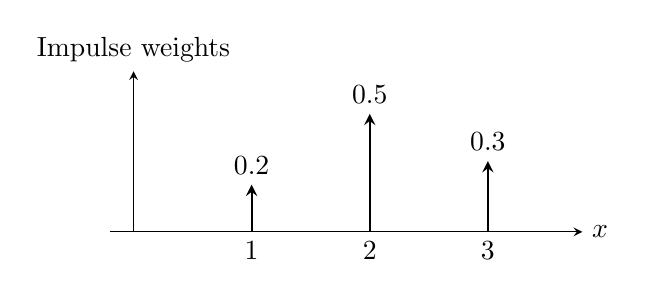
\begin{tikzpicture}[x=1.5cm,y=3cm,>=stealth]
\draw[->](-.2,0)--(3.8,0) node[right]{$x$};
\draw[->](0,0)--(0,.68) node[above]{Impulse weights};
\foreach \x/\p in {1/0.2,2/0.5,3/0.3}{\draw[->,thick](\x,0)--(\x,\p) node[above]{$\p$};\node[below]at(\x,0){$\x$};}
\end{tikzpicture}
\hspace{5mm}
\begin{tikzpicture}[x=1.5cm,y=2.1cm,>=stealth]
\draw[->](-.2,0)--(3.8,0)node[right]{$x$};\draw[->](0,0)--(0,1.25)node[above]{$F_X(x)$};
\draw[thick](0,0)--(1,0);\draw[thick](1,.2)--(2,.2);\draw[thick](2,.7)--(3,.7);\draw[thick](3,1)--(3.65,1);
\foreach \x/\a/\b in {1/0/.2,2/.2/.7,3/.7/1}{\draw[densely dotted](\x,\a)--(\x,\b);\draw[fill=white](\x,\a)circle(1.8pt);\fill(\x,\b)circle(1.8pt);\node[below]at(\x,0){$\x$};}
\foreach \y in {.2,.7,1}{\node[left]at(0,\y){$\y$};}
\end{tikzpicture}
\end{center}
Filled circles indicate included CDF values; open circles indicate excluded endpoints.
\newpage
\problem{1.11}{Suggested}{34}
The density is $f_X(x)=a\ee^{-|x|}$ for $x\in\mathbb R$.
\step{(1) Normalizing coefficient}
A probability density integrates to one. By symmetry,
\[
1=\int_{-\infty}^{\infty}a\ee^{-|x|}\,dx
=2a\int_0^{\infty}\ee^{-x}\,dx=2a.
\]
Therefore
\[
\boxed{a=\frac12},\qquad f_X(x)=\frac12\ee^{-|x|}.
\]
\step{(2) Distribution function}
If $x<0$, then $|t|=-t$ throughout the integration interval, so
\[
F_X(x)=\int_{-\infty}^x\frac12\ee^t\,dt=\frac12\ee^x.
\]
If $x\ge0$, split the integral at zero:
\begin{align*}
F_X(x)&=\int_{-\infty}^0\frac12\ee^t\,dt
+\int_0^x\frac12\ee^{-t}\,dt\\
&=\frac12+\frac12(1-\ee^{-x})=1-\frac12\ee^{-x}.
\end{align*}
Thus
\[
\boxed{F_X(x)=\begin{cases}
\tfrac12\ee^x,&x<0,\\[1mm]
1-\tfrac12\ee^{-x},&x\ge0.
\end{cases}}
\]
Both branches give $F_X(0)=1/2$ by continuity, and the limits at $-\infty$ and $+\infty$ are $0$ and $1$.
\newpage
\problem{1.28}{Suggested}{36}
Use the convention $\phi_X(v)=\E[\ee^{\jj vX}]$. Mutual independence implies
\begin{align*}
\phi_{b+\sum_{k=1}^3a_kX_k}(v)
&=\E\!\left[\ee^{\jj bv}\prod_{k=1}^3\ee^{\jj va_kX_k}\right]\\
&=\ee^{\jj bv}\prod_{k=1}^3\E[\ee^{\jj va_kX_k}]
=\ee^{\jj bv}\prod_{k=1}^3\phi_k(a_kv).
\end{align*}
A coefficient of zero contributes $\phi_k(0)=1$.
\step{(1) $X=X_1+X_2$}
\[
\boxed{\phi_X(v)=\phi_1(v)\phi_2(v).}
\]
\step{(2) $X=X_1+X_2+X_3$}
\[
\boxed{\phi_X(v)=\phi_1(v)\phi_2(v)\phi_3(v).}
\]
\step{(3) $X=X_1+2X_2+3X_3$}
\[
\boxed{\phi_X(v)=\phi_1(v)\phi_2(2v)\phi_3(3v).}
\]
\step{(4) $X=2X_1+X_2+4X_3+10$}
\[
\boxed{\phi_X(v)=\ee^{\jj10v}\phi_1(2v)\phi_2(v)\phi_3(4v).}
\]
Scaling changes the argument of a characteristic function; adding a constant produces a phase factor.
\newpage
\problem{1.29}{Suggested}{36}
Use $\phi(v)=\E[\ee^{\jj vX}]$. The mean-square value is $\E[X^2]$, and
$\Var(X)=\E[X^2]-(\E X)^2$. Discrete densities below use Dirac deltas.
\step{(1) Sum of five exponential terms}
For a discrete variable, $\phi(v)=\sum_k p_k\ee^{\jj vx_k}$.
Thus the five terms give masses $0.2,0.3,0.2,0.2,0.1$ at $0,2,4,-2,-4$:

\[
f_X(x)=0.2\delta(x)+0.3\delta(x-2)+0.2\delta(x-4)
+0.2\delta(x+2)+0.1\delta(x+4).
\]
Consequently,
\begin{align*}
\E X&=0.3(2)+0.2(4)+0.2(-2)+0.1(-4)=\boxed{0.6},\\
\E[X^2]&=0.3(4)+0.2(16)+0.2(4)+0.1(16)=\boxed{6.8},\\
\Var(X)&=6.8-0.6^2=\boxed{6.44}.
\end{align*}
\step{(2) $\phi(v)=0.3\ee^{\jj v}+0.7\ee^{-\jj v}$}
\[
\boxed{f_X(x)=0.3\delta(x-1)+0.7\delta(x+1).}
\]
\[
\boxed{\E X=0.3-0.7=-0.4},\qquad
\boxed{\E[X^2]=1},\qquad\boxed{\Var(X)=1-0.16=0.84}.
\]
\step{(3) $\phi(v)=4/(4-\jj v)$}
Since $\int_0^\infty4\ee^{-4x}\ee^{\jj vx}\,dx=4/(4-\jj v)$,
\[
\boxed{f_X(x)=\begin{cases}4\ee^{-4x},&x\ge0,\\0,&x<0.\end{cases}}
\]
Using $\int_0^\infty x^n\ee^{-4x}\,dx=n!/4^{n+1}$,
\[
\boxed{\E X=\frac14},\qquad\boxed{\E[X^2]=\frac18},\qquad
\boxed{\Var(X)=\frac18-\frac1{16}=\frac1{16}}.
\]
\step{(4) $\phi(v)=\sin(5v)/(5v)$, with $\phi(0)=1$}
The identity $\frac1{10}\int_{-5}^5\ee^{\jj vx}\,dx=\sin(5v)/(5v)$ identifies $X\sim U(-5,5)$:
\[
\boxed{f_X(x)=\begin{cases}\tfrac1{10},&-5\le x\le5,\\0,&\text{otherwise}.\end{cases}}
\]
By symmetry and direct integration,
\[
\boxed{\E X=0},\qquad
\boxed{\E[X^2]=\frac1{10}\int_{-5}^5x^2\,dx=\frac{25}{3}},\qquad
\boxed{\Var(X)=\frac{25}{3}}.
\]
\newpage
\problem{1.30}{Suggested}{36}
Let $X\sim U(a,b)$, where $a<b$. Then
\[
f_X(x)=\begin{cases}\dfrac1{b-a},&a\le x\le b,\\[1mm]0,&\text{otherwise}.\end{cases}
\]
\step{Fourier-transform convention}
For $\mathcal F\{f\}(\omega)=\int_{-\infty}^{\infty}f(x)\ee^{-\jj\omega x}\,dx$,
the characteristic function satisfies
\[
\phi_X(v)=\int_{-\infty}^{\infty}f_X(x)\ee^{\jj vx}\,dx
=\mathcal F\{f_X\}(-v).
\]
\step{Evaluate the transform}
For $v\ne0$,
\begin{align*}
\phi_X(v)&=\frac1{b-a}\int_a^b\ee^{\jj vx}\,dx\\
&=\frac{\ee^{\jj vb}-\ee^{\jj va}}{\jj v(b-a)}\\
&=\ee^{\jj v(a+b)/2}\,
\frac{\sin\!\left(v(b-a)/2\right)}{v(b-a)/2}.
\end{align*}
At $v=0$, $\phi_X(0)=\int f_X(x)\,dx=1$, also obtained by taking the limit.
Therefore
\[
\boxed{\phi_X(v)=\begin{cases}
\displaystyle\ee^{\jj v(a+b)/2}\frac{\sin\!\left(v(b-a)/2\right)}{v(b-a)/2},&v\ne0,\\[3mm]
1,&v=0.
\end{cases}}
\]
\step{Common special cases}
For $X\sim U(-A,A)$ with $A>0$,
\[
\phi_X(v)=\frac{\sin(Av)}{Av},\qquad\phi_X(0)=1.
\]
For $X\sim U(0,A)$,
\[
\phi_X(v)=\ee^{\jj vA/2}\frac{\sin(vA/2)}{vA/2},\qquad\phi_X(0)=1.
\]
\end{document}
